\section{Shift register con D-latch}
Si è montato uno shift register a 4 bit utilizzando 2 integrati 74LS74 che contengono 2 FF D-Latch ciascuno come in \fig{shift}. Le resistenze utilizzate sono da \SI{330}{\ohm}.

	\begin{figure}[h!]

	\end{figure}
	
\begin{figure}[h!]
	\centering
	\begin{minipage}{0.49\textwidth}
		\centering
		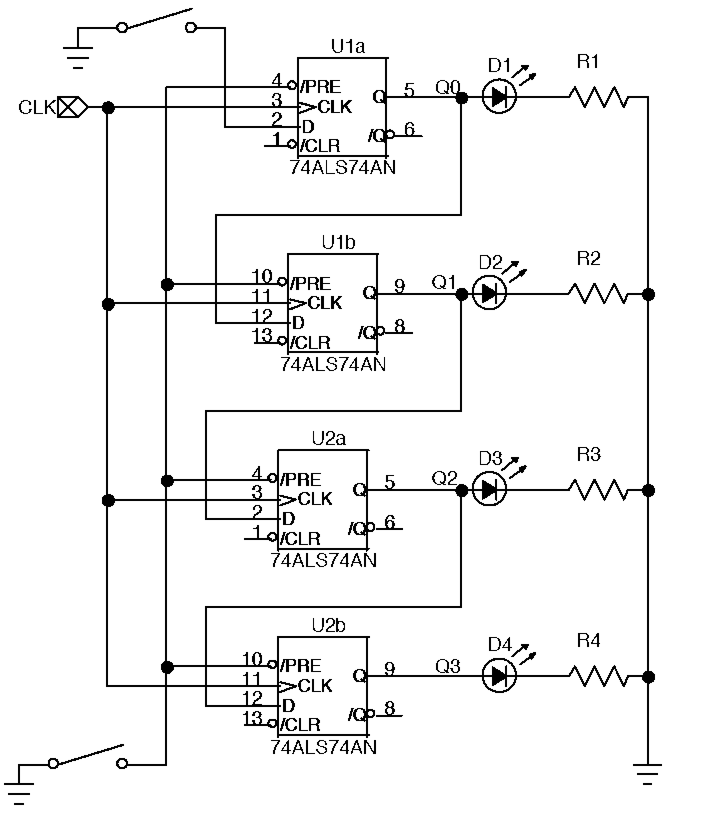
\includegraphics[scale=0.41]{shift.png}
		\caption{Schema dello shift register}
		\label{fig:shift}
	\end{minipage}
	\begin{minipage}{0.49\textwidth}
		\centering
		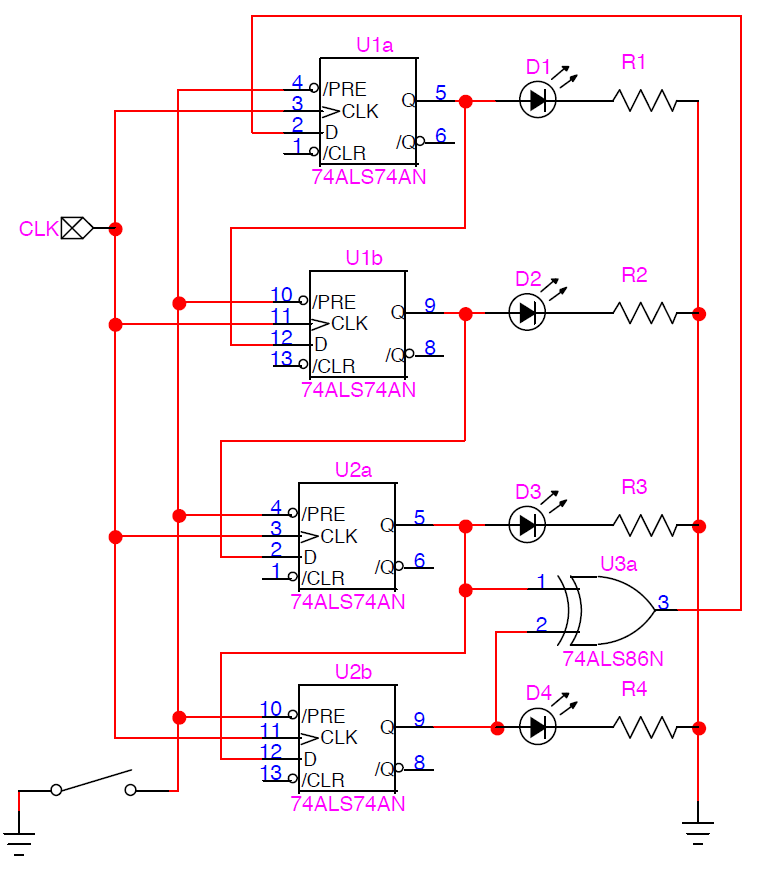
\includegraphics[scale=0.39]{random.png}
		\caption{Schema del generatore pseudocasuale}
		\label{fig:random}
	\end{minipage}
\end{figure}
Gli ingressi CLR e PRE sono stati lasciati disconnessi senza osservare malfunzionamenti e rendendo quindi non necessarie le resistenze di pull-up.

Si è quindi proceduto ad inviare un clock a bassa frequenza (dell'ordine di $\sim\SI{1}{\hertz}$) per verificare il funzionamento del circuito: il bit inviato attraverso l'interruttore al primo D-Latch si propaga nei successivi ad ogni periodo di clock.
Lo stato delle uscite dopo aver premuto il pulsante di preset è HIGH, come atteso.
 
\section{Generatore di sequenze pseudo-casuali}
Si vuole realizzare un generatore di sequenze pseudo casuali a partire dallo shift register prima realizzato. Si sono collegati i due bit più significativi (Q2 e Q3: le uscite degli ultimi due D-Latch, che quindi hanno il ruolo di tap) ad una porta XOR, la cui uscita è stata collegata all'ingresso del primo D-Latch.
Si è quindi chiuso l'interruttore di preset e con un clock a bassa frequenza si è lasciato evolvere l'output. In \fig{random} è riportato lo schema modificato del circuito.
Di seguito si riporta la sequenza osservata in un ciclo:

\begin{equation*}
\begin{matrix}
1.	\qquad	1	&	1	&	1	&	1	\\
2.	\qquad	0	&	1	&	1	&	1	\\
3.	\qquad	0	&	0	&	1	&	1	\\
4.	\qquad	0	&	0	&	0	&	1	\\
5.	\qquad	1	&	0	&	0	&	0	\\

\end{matrix}
\qquad \qquad
\begin{matrix}

6.	\qquad	0	&	1	&	0	&	0	\\
7.	\qquad	0	&	0	&	1	&	0	\\
8.	\qquad	1	&	0	&	0	&	1	\\
9.	\qquad	1	&	1	&	0	&	0	\\
10.	\qquad	0	&	1	&	1	&	0	\\
\end{matrix}
\qquad \qquad
\begin{matrix}

11.	\qquad	1	&	0	&	1	&	1	\\
12.	\qquad	0	&	1	&	0	&	1	\\
13.	\qquad	1	&	0	&	1	&	0	\\
14.	\qquad	1	&	1	&	0	&	1	\\
15.	\qquad	1	&	1	&	1	&	0	\\
\end{matrix}
\end{equation*}

Non esistono altri tap capaci di generare una sequenza di lunghezza massima, come riportato in \href{http://www.physics.otago.ac.nz/reports/electronics/ETR2012-1.pdf}{http://www.physics.otago.ac.nz/reports/electronics/ETR2012-1.pdf}.
In questo documento si fa riferimento all'uso di porte XNOR, tuttavia il circuito è del tutto equivalente a patto di modificare la sequenza iniziale. Si da per buono che l'uscita della porta logica debba essere Q0, differentemente il primo bit non modificherebbe mai il proprio valore.

